\section{Introdução e Justificativa}
\label{sec:int}

Os avanços tecnológicos de sistemas distribuídos estão permitindo que as pessoas utilizem serviços com volumes massivos de dados para aplicações sensíveis a latência.
%
Essa situação é propícia à área de jogos massivos, e tem atraído pesquisadores para essa área de estudo~\cite{mmo_analytic,1417630,6267019,6063041}.
%
O principal objetivo destas pesquisas é reduzir a carga e o impacto a latência para o usuário final nesses serviços.
%
Reduzir a carga e impacto da latência em serviços para jogos massivos resulta em uma melhor experiência de jogabilidade aos usuários finais~\cite{1417630}.


Jogos \ac{MMORPG} são utilizados como negócio viável e lucrativo, sendo a experiência de jogabilidade na qual o usuário final será submitido é um fator crítico para o sucesso.
%
O mercado de jogos \ac{MMORPG} vem crescendo desde 2012~\cite{new_york_times}, sendo no ano de 2016 um dos mais lucrativos~\cite{statista_2016}.
%
A sua projeção para 2018 é que sejam arrecadados mais de 30 bilhões de dólares americanos com esta categoria de jogos~\cite{statista_2018}, um aumento de 20\% a mais sobre o ano de 2016.



\ac{MMORPG} são jogos de interpretação de papéis massivos.
%
A principal característica desse estilo de jogo é a comunicação e representação virtual de um mundo fantasia no qual cada jogador pode interagir com objetos virtuais compartilhados ou tomar ações sobre outros de jogadores em tempo real, tendo como principais objetivos a resolução de problemas conforme a sua regra de \textit{design}, o desenvolvimento do personagem e a interação entre os jogadores\cite{video_game_technologies}.
%

Um jogo \ac{MMORPG} é arquitetado em duas partes~\cite{mmo_analytic}:
\begin{itemize}
  \item \textbf{Serviço}: É o macrosserviço que implementa as regras de negócio e requisitos do jogo.
  O serviço disponibiliza uma interface com ações possíveis ao cliente sobre algum protocolo de rede.
  \item \textbf{Cliente}: Cliente é a aplicação que realizará as requisições com a interface do macrosserviço, exibindo o estado de jogo de forma imersiva ao jogador.
\end{itemize}

A maioria dos jogos \ac{MMORPG} disponíveis no mercado estão implementados sobre uma arquitetura que executa sobre diversos servidores\cite{stephenclarkewillson2017}, nos quais o desempenho destes servidores influencia tanto na experiência de jogabilidade do usuário final, quanto no custo de manutenção destes serviços~\cite{1417630}.
%
Modelar um sistema de alto desempenho torna-se um trabalho essencial para a satisfação do usuário final~\cite{1417630}.
%
As ocorrências geradas por um sistema de baixo desempenho podem acarretar em frustração do usuário com o serviço e/ou aumento dos gastos com recurso computacional para manter o serviço.
%
Uma ocorrência é qualquer tipo de mal funcionamento em uma aplicação, não necessariamente aparente ao usuário final~\cite{1417630}.
%
Evitar ou eliminar as ocorrências durante o projeto e desenvolvimento das arquiteturas do serviço é um processo crítico para o bom funcionamento desses jogos.

\subsection{Ocorrências de serviços massivos}
\label{sec:ocorrencias}

Uma métrica popular para mensurar o desempenho de um serviço \ac{MMORPG} é o número de conexões~\cite{1417630} simultâneas suportadas.
%
Em geral, caso o serviço ultrapasse o limite para o qual este foi projetado, diversas falhas de conexão, problemas de lentidão ou dessincronização com o cliente podem ocorrer.
%
Neste contexto, as ocorrências comuns são~\cite{1417630}:

\begin{itemize}
  \item \textbf{Longo tempo de resposta aos clientes}: implica em uma qualidade insatisfatória de jogabilidade ao usuário ou até mesmo impossibilitando o uso do serviço.
  \item \textbf{Dessincronização com os clientes}: realiza reversão na aplicação. Reversão é definida pela situação na qual uma requisição é solicitada ao servidor, um pré-processamento aparente é executado e essa requisição é negada, sendo necessário desfazer o pré-processamento aparente realizado ao cliente.
  \item \textbf{Problemas internos ao serviço}:  podem estar relacionados a diversos outros erros internos de implementação ou a capacidade de recurso computacional (\textit{e.g.,} sobrecarga no banco de dados, gerenciamento lento do espaço ou inconsistências dentro do jogo perante a regra de negócios).
  \item \textbf{Falha de conexão entre o cliente e os microsserviços}: causa a negação de serviço ao usuário final.
\end{itemize}

Existem algumas causas comuns para essas as ocorrências descritas~\cite{1417630}:

\begin{itemize}
  \item \textbf{Baixo poder computacional do servidor}: poder computacional baixo para a qualidade de experiência de jogabilidade do usuário final desejada.
  \item \textbf{Complexidade de algoritmos}: o serviço usa algoritmos de alta complexidade ou regras de negócios que demandam por um algoritmo complexo.
  \item \textbf{Limitado pela própria arquitetura}: está limitado diretamente pelo número de conexões, não suportando a carga recebida.
\end{itemize}

Tais ocorrências estão diretamente correlacionadas a carga a qual tais serviços estão submetidos e podem ser amenizadas utilizando técnicas de provisionamento de recursos e balanceamento de carga~\cite{1417630}, mas não suficiente para eliminar tais ocorrências.

A área de desenvolvimento web compartilha várias ocorrências comuns geradas por sobrecarga do serviço~\cite{7830692}.
%
Em desenvolvimento web é comum utilizar a abordagem de microsserviços para resolver o problema de sobrecarga, modularizando o  funcionamento em módulos menores.
%
Da mesma forma, faz sentido modularizar um serviço \ac{MMORPG} em microsserviços para suportar cargas maiores e diminuir o custo de manutenção~\cite{7515686}.

\subsection{Arquiteturas de microsserviços}

Entende-se por microsserviço as aplicações que executam operações menores de um macrosserviço, da melhor forma possível~\cite{stephenclarkewillson2017}.
%
Microsserviços devem funcionar separadamente e de forma autônoma.
%
Seu funcionamento deve ser desenhado para permitir alinhamentos de alta coesão e baixo acoplamento entre os demais microsserviços existentes em um macrosserviço~\cite{8169955}.



Arquiteturas de microsserviços iniciam uma nova linha de desenvolvimento de aplicações preparadas para executar sobre nuvens computacionais, promovendo maior flexibilidade, escalabilidade, gerenciamento e desempenho, sendo a principal escolha de arquitetura de grandes empresas como Amazon, Netflix e LinkedIn~\cite{7830692,7515686}.
%
Um microsserviço é definido pelas seguintes características~\cite{8169955}:

\begin{itemize}
  \item Deve posibilitar a implementação como uma peça individual do macrosserviço.
  \item Deve funcionar individualmente.
  \item Cada serviço deve ter uma interface. Essa interface deve ser o suficiente para utilizar o microsserviço.
  \item A interface deve estar disponível na rede para chamada de processamento remoto.
  \item O serviço pode ser utilizado por qualquer linguagem de programação e/ou plataforma.
  \item O serviço deve executar com as dependências mínimas.
  \item Ao agregar vários microsserviços, o macrosserviço resultante poderá prover funcionalidades complexas.
\end{itemize}

Alguns exemplos de arquitetura de microsserviços para jogos \ac{MMORPG} são as arquiteturas apresentadas por Rudy (Figura~\ref{fig:rudy}), Salz (Figura~\ref{fig:salz}) e a arquitetura escrita por Knowles (Figura~\ref{fig:knowles}).

\begin{figure}[htb!]
  \begin{minipage}{.5\textwidth}
    \caption{Arquitetura Rudy, utilizada no jogo Tibia.}
    \label{fig:rudy}
    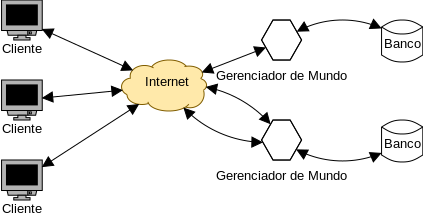
\includegraphics[height=3.5cm]{arquiteturas/rudy.png}
    \centering

    Adaptado de:~\cite{matthiasrudy2011}
  \end{minipage}
  \begin{minipage}{.5\textwidth}
    \caption{Arquitetura Salz, utilizada no jogo Albion.}
    \label{fig:salz}
    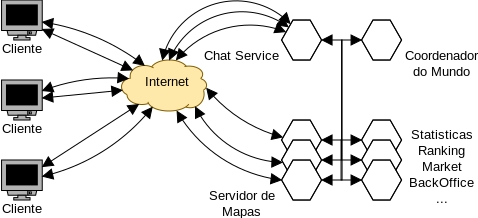
\includegraphics[height=3.5cm]{arquiteturas/salz.png}
    \centering

    Adaptado de:~\cite{albion_online_unite}
  \end{minipage}%
\end{figure}

\begin{figure}[htb!]
  \caption{Arquitetura Knowles, utilizada no jogo Guild Wars 2.}
  \label{fig:knowles}
  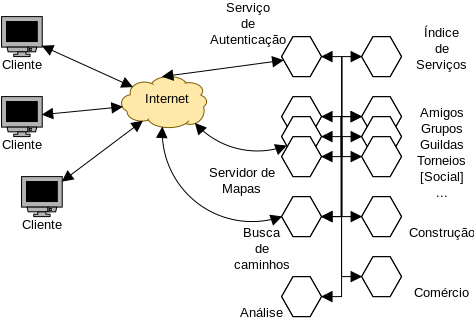
\includegraphics[height=5.5cm]{arquiteturas/knowles.png}
  \centering

  Adaptado de:~\cite{stephenclarkewillson2017}
\end{figure}

A arquitetura Rudy (Figura~\ref{fig:rudy}) é formada por um sistema cliente-servidor monolítico, na qual cada microsserviço individual gerencia um mundo mútuo dos demais gerenciadores de mundo~\cite{matthiasrudy2011}.
%
Essa arquitetura dificulta a escalabilidade, modificações e manutenção~\cite{8169955}, além de segregar a comunidade de jogadores em servidores menores~\cite{matthiasrudy2011}.
%
Inicialmente essa arquitetura foi pensada para ser um sistema Cliente-Servidor monolítico.
%
A arquitetura Rudy é uma arquitetura de microsserviços adaptada de um serviço cliente-servidor~\cite{matthiasrudy2011}.
%
O jogo Tibia\footnote[1]{Tibia: \url{http://www.tibia.com}}, operante sobre essa arquitetura, possui 68 mundos oficiais (Sendo 2 servidores de teste)~\cite{matthiasrudy2011}, com capacidade para 1.050 clientes em cada servidor, na qual encontra-se restringido pelo gerenciador de mundo.



A arquitetura Salz (Figura~\ref{fig:salz}) é formada por diversos microsserviços~\cite{albion_online_unite}.
%
O principal objetivo dessa arquitetura é modularizar o serviço visando melhorar a escalabilidade.
%
Ela é atualmente utilizada no jogo Albion Online\footnote[2]{Albion Online: \url{https://albiononline.com}}.
%
A arquitetura é planejada para funcionar conforme a seguinte especificação\cite{albion_online_unite}:

\begin{itemize}
  \item O mundo é distribuído sobre os vários servidores de mapas. Cada microsserviço gerencia uma região do mundo, denominado \textit{chunk}.
  \item Jogadores mudam a conexão com os microsserviços quando estão posicionados na borda de um \textit{chunk}.
  \item A autorização de acesso aos microsserviços é obtido pelo banco de dados.
  \item O coordenador do mundo é responsável por tudo que seja de escopo global (\textit{e. g.,} Grupos, chat global, guildas, \textit{etc.}).
\end{itemize}

A arquitetura Knowles (Figura~\ref{fig:knowles}) é distribuída em diversos microsserviços, assim como a arquitetura Salz (Figura~\ref{fig:salz}).
%
A diferença em comparação a arquitetura Salz (Figura~\ref{fig:salz}) está na decomposição da arquitetura para outros microsserviços e a conexão direta entre esses microsserviços e o cliente.
%
O principal objetivo dessa arquitetura é facilitar a manutenção e desempenho de reinicialização do macrosserviço~\cite{stephenclarkewillson2017}.
%
Guild Wars 2\footnote[3]{Guild Wars 2: \url{https://www.guildwars2.com}} é um jogo que executa sobre a arquitetura Knowles.
%
Ele é popularmente conhecido por ter seus serviços sempre ativos, visto que a arquitetura possibilita desativar pequenos pedaços do serviço para manutenções básicas e a sua reinicialização é rápida para manutenções críticas.

Conforme as arquiteturas de microsserviços dos jogos \ac{MMORPG} aumentam para atender novas demandas do mercado, o seu custo computacional e complexidade de nós na nuvem computacional aumentam.
%
Por esse motivo a análise e otimização dessas arquiteturas é importante para impactar em um melhor desempenho tanto ao usuário final, quanto a otimização de lucros das empresas que disponibilizam esses serviços.

\subsection{Justificativa}

A proposta de otimização das análises realizadas sobre as arquiteturas de microsserviços para jogos massivos focada ao gerenciamento de mundos virtuais, proposta pela literatura, traz impacto direto ao usuário final e a empresa que mantem esse sistema~\cite{1417630}.

A proposta contida no atual trabalho visa indentificar meios para otimizar tais arquiteturas, visando melhorar algumas características específicas:

\begin{itemize}
  \item Recursos utilizados.
  \item Escalabilidade.
  \item Disponibilidade.
  \item Flexibilidade.
\end{itemize}
